\newpage
\thispagestyle{sectioned}
\chapter{Arquitectura de DemoCritics}

\section{Arquitectura de Wave}

\section{Arquitectura de la aplicación}

La arquitectura está compuesta por cuatro módulos principales de los que hablaremos en profundidad en las siguientes subsecciones. Como \textbf{Cliente móvil} tendremos la aplicación desarrollada en Android, que realizará peticiones HTTP al servicio web alojado en OpenShift \cite{ref:OpenShift}, una plataforma que permite alojar servicios web de forma gratuita. Dentro del servicio contaremos con una \textbf{API RESTful} que será quien gestione las peticiones de la aplicación móvil mediante el protocolo HTTP.

CAMBIAR FOTO PARA VER INTEGRACION CON WAVE

\begin{figure}[H]
\centering
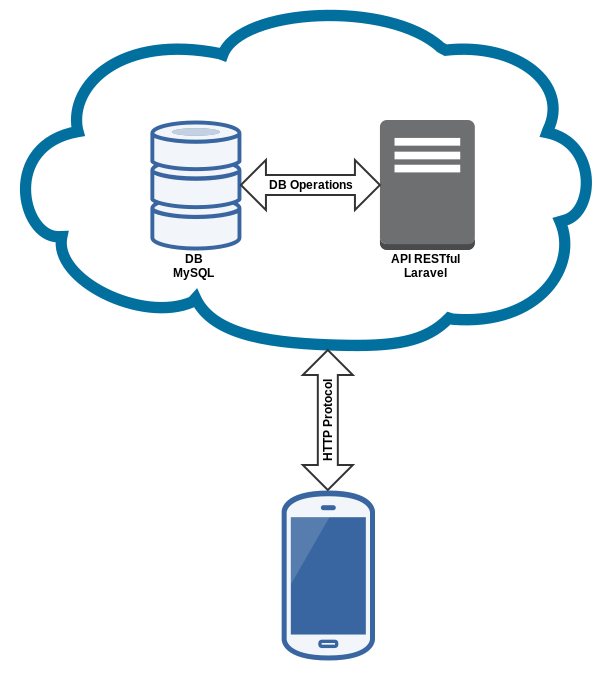
\includegraphics[keepaspectratio, scale=0.4]{Media/Captures/architecture.png}
\caption{Arquitectura de la aplicacción.}
\label{fig:architecture}
\end{figure}

Por otro lado, la aplicación hará uso del \textbf{Servicio Android} desarrollado en SwellRT-Android \cite{ref:swellRT_android_github} para conectarse con el servidor Wave alojado en https://wave.p2pvalue.eu/ e intercambiar los datos que sea necesario mantener en tiempo real, es decir, la edición de una Propuesta de forma colaborativa entre varias personas.

Por último, la \textbf{Base de Datos MySQL} alojada en el servidor de OpenShift almacenará toda la información relacionada con la aplicación. La API RESTful será quien actúe de intermediario entre las peticiones de la aplicación y las operaciones en Base de Datos.

\subsection{Back-end}

\subsubsection{Base de Datos}\label{sssec:database}

En la implementación de la Base de Datos se ha utilizado un Modelo Relacional para la definición de las tablas. Utilizando MySQL \cite{ref:MySQL} como sistema de gestión de base de datos (SGBD) y phpMyAdmin \cite{ref:phpMyAdmin} como herramienta de gestión gráfica de la base de datos.

La base de datos está formada por un total de 12 tablas donde se almacena toda la información relacionada con los programas de los partidos políticos, las propuestas ciudadanas, encuestas, comparativas... y otros datos más técnicos como la gestión de los usuarios, la relación de los comentarios o la relación entre las secciones y comparativas entre otras.

\begin{figure}[H]
\centering
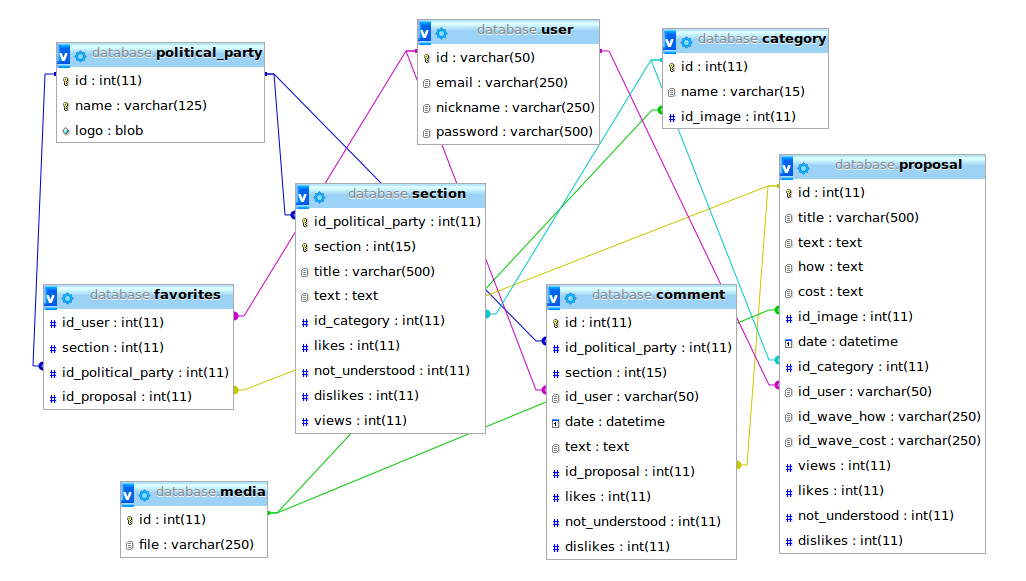
\includegraphics[keepaspectratio, scale=0.30]{Media/Captures/database.png}
\caption{Modelo entidad-relación de la base de datos.}
\label{fig:ermodel}
\end{figure}

Las tablas \textit{section} y \textit{political-party} son utilizadas para guardar información estática en la aplicación. Es decir, en la tabla \textit{political-party} se almacenan los partidos políticos que se presentan a unas elecciones, y en la tabla \textit{section}, las diferentes secciones de un programa electoral. Tan sólo modificaremos las columnas de \textit{likes}, \textit{dislikes}, \textit{not-understood} y \textit{views} para obtener estadísticas de uso de cada sección. El resto de las columnas permanecerán intactas.

EXPLICAR RESTO DE TABLAS. DATOS ESTATICOS VS DINAMICOS

Las demás tablas serán utilizadas para guardar datos dinámicos de la aplicación. Datos que normalmente genera un usuario visitando una sección de un programa, creando una propuesta, haciendo un comentario, etc.

\subsubsection{Service REST}\label{sssec:rest}

Para establecer la conexión de la aplicación desarrollada en Android con la Base de Datos hemos utilizado \textbf{Laravel} como Servicio Web. Laravel \cite{ref:laravel} es un framework de código abierto para desarrollar aplicaciones web con PHP 5. Laravel permite además montar una API REST (Representational State Transfer), un estilo de arquitectura software para sistemas hipermedia distribuidos como la World Wide Web. Este término se originó en una tesis doctoral sobre la web escrita por Roy Fielding \cite{ref:RESTPhd}.

Laravel nos permite implementar un sistema RESTful para que el cliente móvil pueda hacer peticiones al servicio web y que dicho servicio responda a éstas de la forma que queramos. Estas peticiones se realizan mediante el protocolo HTTP. En función de la operación que deseemos hacer, haremos distintos tipos de petición;

\begin{itemize}
	\item GET: para obtener datos de la Base de Datos.
	\item POST: para modificar datos de la Base de Datos.
	\item PUT: para insertar datos en la Base de Datos.
	\item DELETE: para borrar datos de la Base de Datos.
\end{itemize}

YO NO PONDRIA ESTA FOTO, DEMASIADO BLANCA Y NO APORTA NADA 

\begin{figure}[H]
\centering
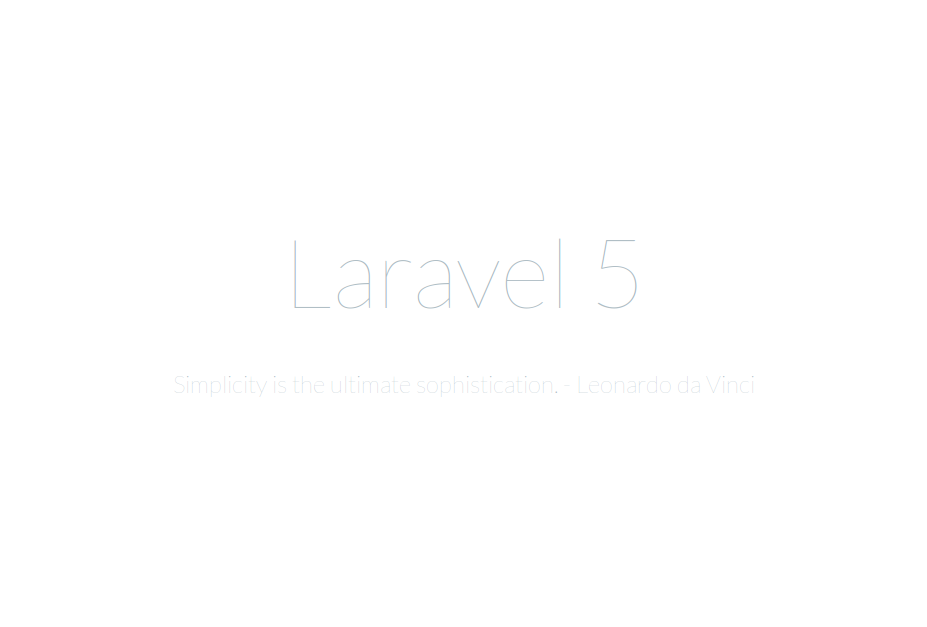
\includegraphics[keepaspectratio, scale=0.30]{Media/Captures/laravel5.png}
\caption{Pantalla principal de Laravel 5.}
\label{fig:laravel5}
\end{figure}

Usar un servicio RESTful nos proporciona una gran flexibilidad a la hora de independizar la tecnología del servidor de la del cliente. Mediante la arquitectura basada en peticiones HTTP no solo podremos hacer peticiones desde el cliente en Android, sino que más adelante podriamos desarrollar una versión web o incluso un cliente para iOS sin tener que modificar el servicio, ya que las peticiones HTTP serán las mismas.

Para organizar las diferentes peticiones en función de su uso, Laravel proporciona una estructura en forma de API que basa su funcionamiento en dos elementos: el archivo de Rutas (Routes.php) y los controladores (Controller.php).

El Routes se organiza...

Los controllers... -> CONSULTA DE BASE DE DATOS

ORGANIZACION DE ROUTES Y CONTROLLERS

DEVOLVER JSON

EJEMPLOS DE URL Y RESULTADO

\subsubsection{Servicio Android de conexión con Wave}

REORDENAR LO DE WAVE

\subsection{Front-end: Cliente Android}

INTERFAZ GRAFICA -> PRESENTACION AL USUARIO

ARQUITECTURA DE PETICIONES AL REST

ARQUITECTURA DE PETICIONES A WAVE

